

\section{Grundlagen}
In diesem Kapitel werden die verschiedenen Grundlagen für die Steuerungsarten erklärt.
\subsection{Phasenanschnittsteuerung}
Bei der Phasenanschnittsteuerung wird das Sinussignal über einen TRIAC geführt. Ein TRIAC sind zwei antiparallel geführt Thyristoren. Dieser zündet ab einem gewissen Zündimpuls nach jedem Nulldurchgang. Je später der TRIAC eingeschaltet wird, desto kleiner wird die mittlere Leistung über der Last. Ein Vorteil gegenüber einem Spannungsteiler ist, dass weniger Leistung gebraucht wird. Der Zündwinkel kann von 0\textdegree bis 180\textdegree gewählt werden, wobei bei 0\textdegree die maximale Leistung und bei 180\textdegree keine Leistung über der Last anliegt. Das Problem bei der Phasenanschnittsteuerung ist, dass diese Schaltung Oberwellen verursacht und so ungewünschte Effekte für den Netzbetreiber verursacht. Ein weiteres Problem betrifft den nicht-sinusförmigen Stromverlauf. Da Strom und Spannung nicht den gleichen Verlauf haben, tritt eine Verzerrungsblindleistung auf.  Der Strom verläuft zeitlich der Spannung nach wirkt so wie eine Induktivität. Deshalb wird dieses Verfahren vom EW nur bei kleinen Leistungen toleriert. Bei grossen Leistungen wird deshalb die Schwinungspaketsteuerung benutzt. In der Abbildung \ref{fig:Phasenanschnitt} ist erischtlich, wie der Phasenanschnitt bei einer Netzspannung aussieht. Grau gezeichnet ist die normale Netzspannung und rot ist die Spannung welcher an der Last anliegt. In dieser Abbildung wurde ein Winkel von 135\textdegree gewählt und somit ist die Leistung an der Last kleiner als mit der normalen Netzspannung. 

\begin{figure}[ht!]
	\centering
	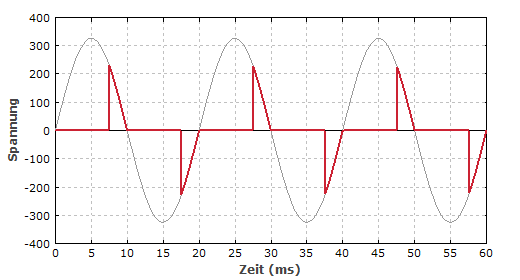
\includegraphics[scale=0.75]{phasenanschnittsteuerung1.png}	
	\caption{Phasenanschnitt mit einem Winkel von 135\textdegree \cite{Phasenanschnittsteuerung}}\label{fig:Phasenanschnitt1}
\end{figure}
\newpage
\begin{figure}[ht!]
	\centering
	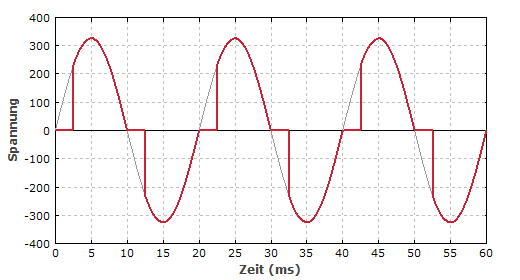
\includegraphics[scale=0.75]{phasenanschnittsteuerung2.png}	
	\caption{Phasenanschnitt mit einem Winkel von 45\textdegree \cite{Phasenanschnittsteuerung}}\label{fig:Phasenanschnitt2}
\end{figure}
Bei der Abbildung \ref{fig:Phasenanschnitt2} ist gut ersichtlich, wie früher gezündet wurde. Somit wird die Leistung an der Last grösser.

\subsection{Schwingungspaketsteuerung}
In diesem Verfahren wird nicht wie der Phasenanschnittsteuerung die Form der Halbwellen verändert, sondern die Zeitdauer. Dabei wird immer von der Paketzeit und der Einschaltzeit ausgegangen, wobei letzteres verändert wird. Wenn z.B. eine Paketdauer 10 Halbwellen hat, und die Einschaltdauer 5 Halbwellen ist, liegt die halbe Leistung über der Last an. Anders als bei der Phasenanschnittsteuerung enstehen bei dieser Ansteuerungsart keine harmonische Oberwellen, dafür aber Sub- und Zwischenharmonische. Auf der Abbildung \ref{fig:Schwingungspaketsteuerung} ist ersichtlicht, wie vier von den total sechs pro Paket eingeschaltet sind. Dies ergibt eine Leistung welche ${2}/{3}$ so gross ist wie die Leistung mit der normalen Netzspannung.

\begin{figure}[ht!]
	\centering
	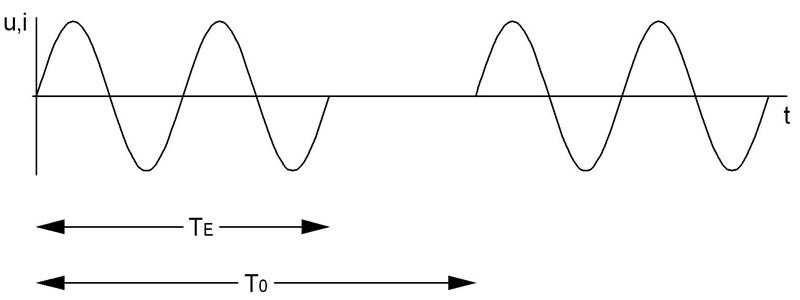
\includegraphics[scale=0.5]{Schwingungspaketsteuerung.png}	
	\caption{Schwingungspaketsteuerung ${2}/{3}$ der Leistung \cite{Schwingungspaketsteuerung}}\label{fig:Schwingungspaketsteuerung}
\end{figure}

Dabei ergibt sich aus dem Verhältnis von Einschaltdauer zu Periodendauer das Tastverhältnis.

\begin{equation}
\lambda = \frac{T_E}{T_0}
\end{equation}



\subsection{Leistungsfaktor}

\begin{figure}[ht!]
	\centering
	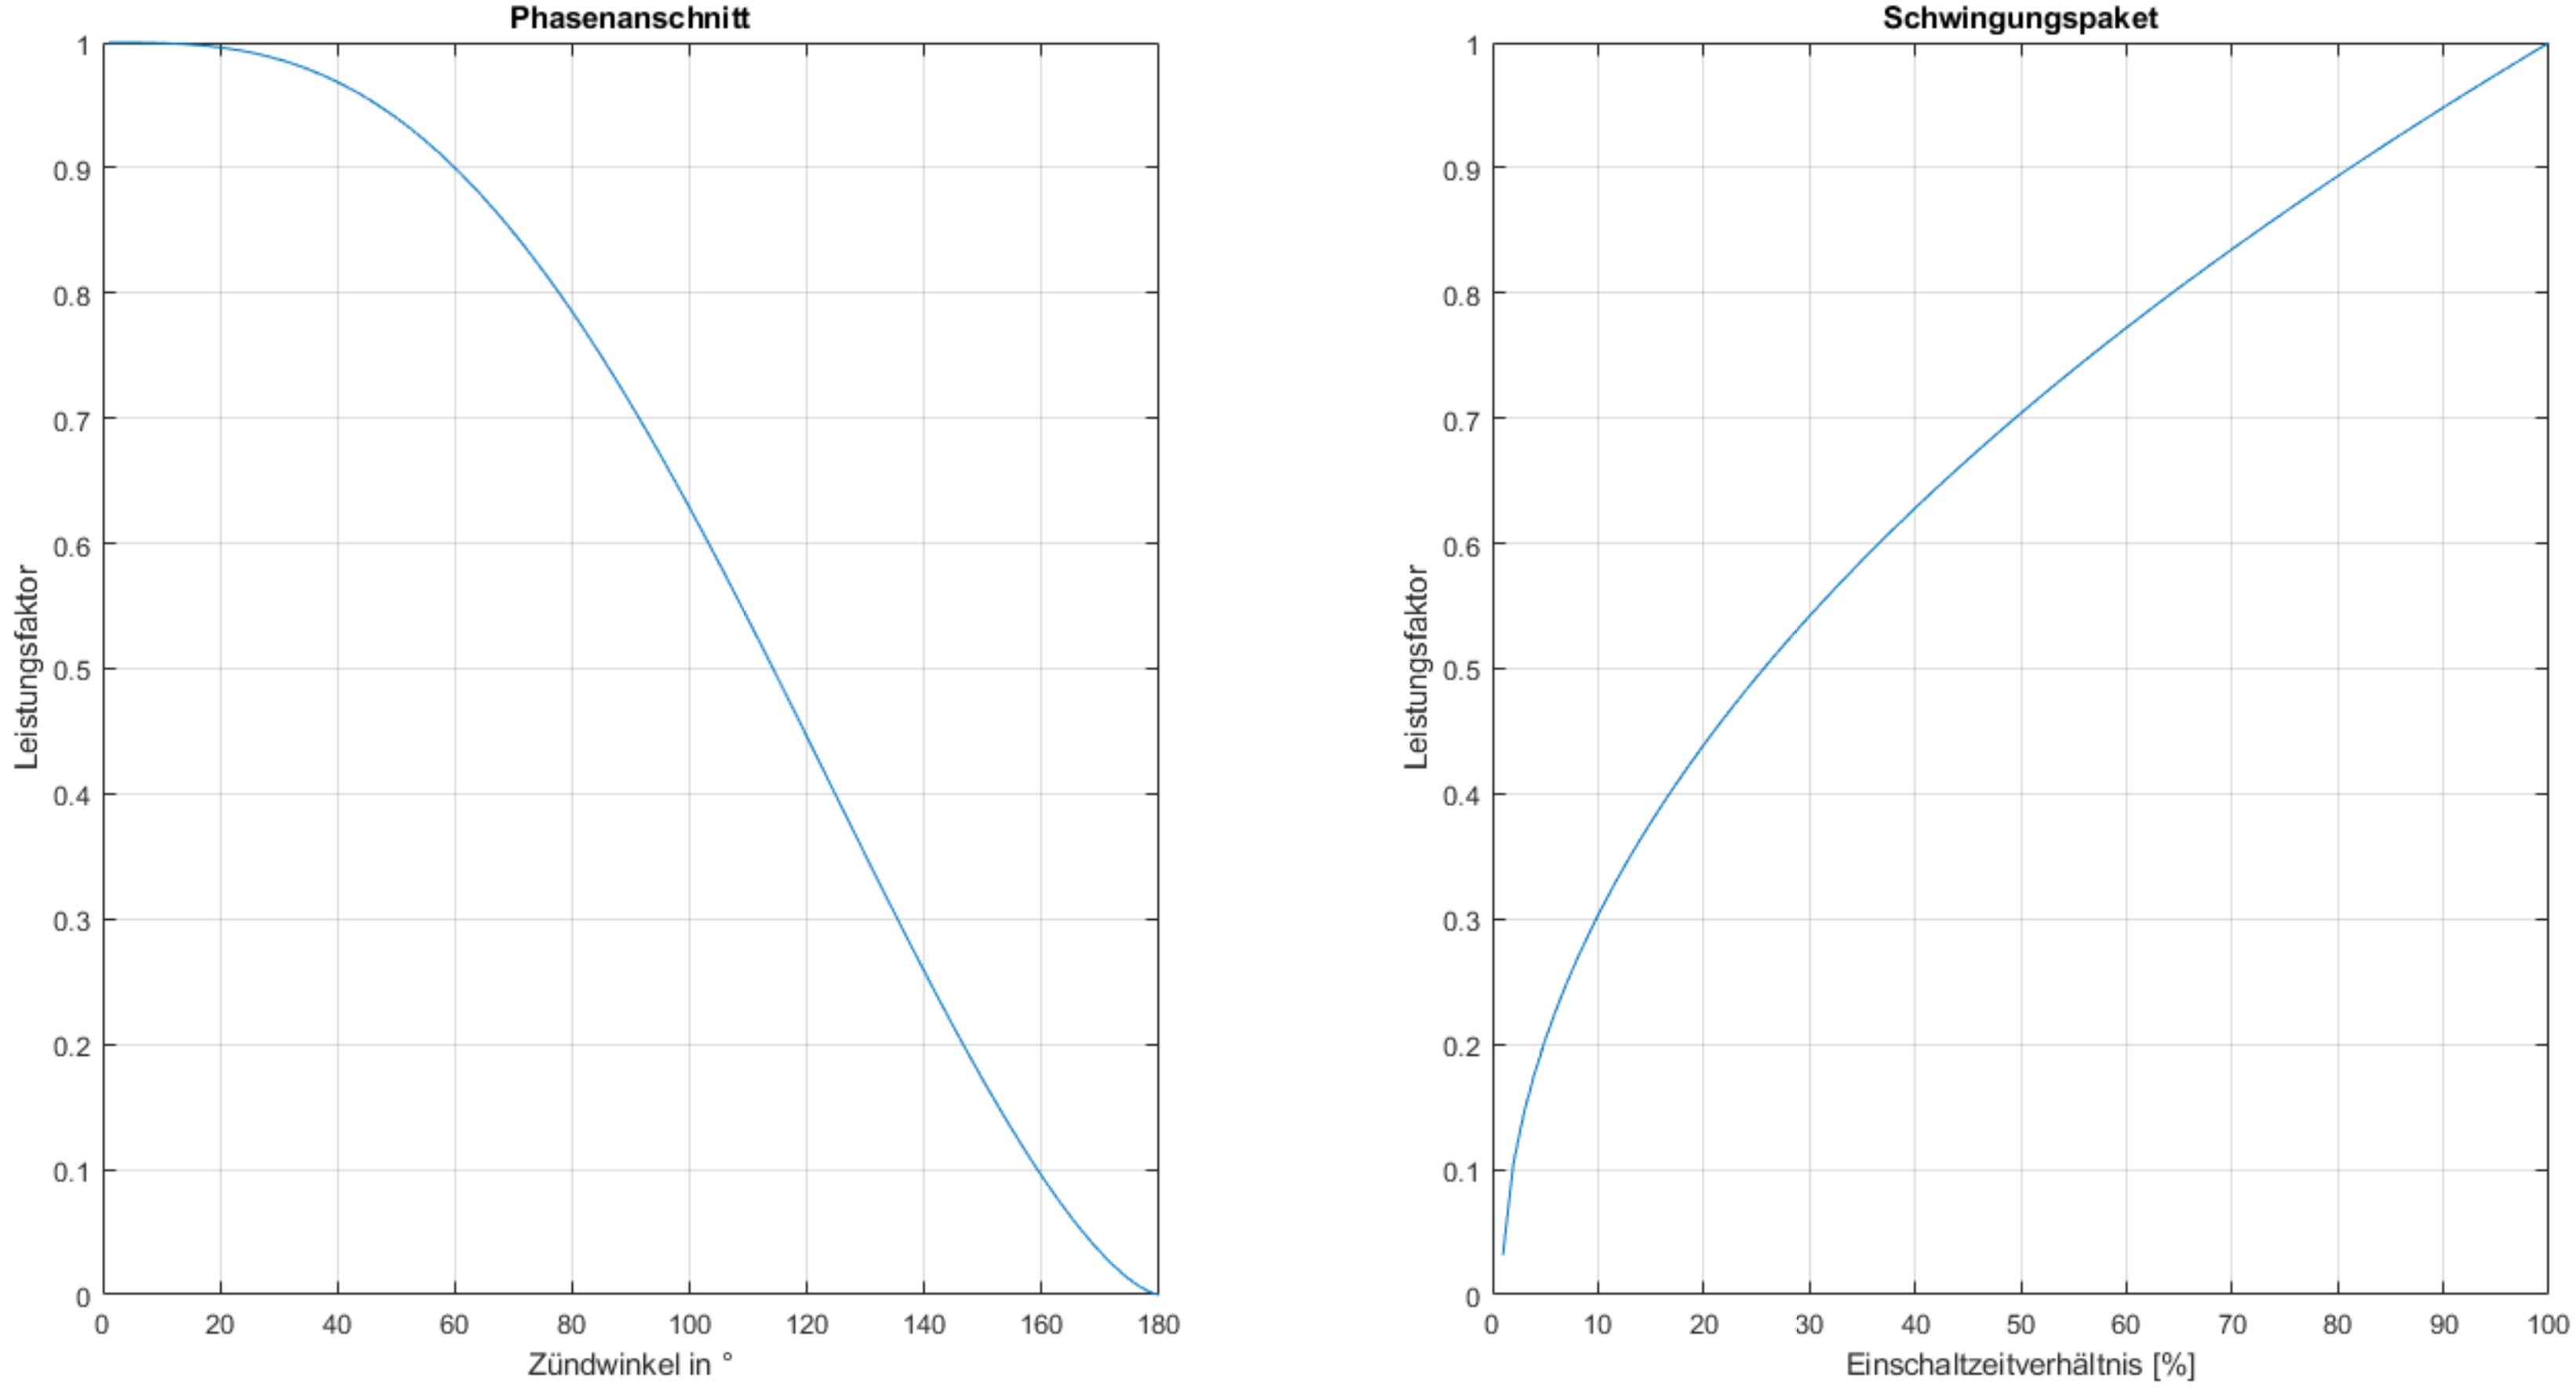
\includegraphics[scale=0.394]{Leistungsfaktor.png}	
	\caption{Leistungsfaktor von Phasenanschnitt- und Schwingungspaketsteuerung}\label{fig:Leistungsfaktor}
\end{figure}

\subsubsection{Leistungsfaktor Phasenanschnittsteuerung}
Der Leistungsfaktor ist definiert als das Verhältnis von Wirkleistung zu Scheinleistung. 
\begin{equation}\label{eq:lamda_p}
\lambda = \frac{P_{\alpha}}{S}
\end{equation}
Die Schein- und Wirkleistung können mit den folgenden Formeln beschrieben werden.
\begin{equation}\label{eq:Schein-&Wirkleistung}
\begin{array}{cc} 
S = I_L \cdot U_{UN}   &   P_{\alpha} = I_L^2 \cdot R_L  \\
\end{array}
\end{equation}
Werden die Formeln \ref{eq:Schein-&Wirkleistung} in die Formel \ref{eq:lamda_p} eingesetzt ergibt sich folgende Gleichung. 
\begin{equation} \label{eq:Phas_1}
\frac{P_{\alpha}}{S} = \frac{I_L \cdot R_L}{U_{UN}}
\end{equation}
Der Laststrom wird mit folgender Formel beschrieben.
\begin{equation}
I_L = \sqrt{1-\frac{\alpha}{\pi}+\frac{1}{2\pi} \cdot sin(2\alpha)} \cdot \frac{U_{UN}}{R_L}
\end{equation}
Wenn die Formel für den Laststrom in die Gleichung \ref{eq:Phas_1} eingesetzt wird, lassen sich die Spannung und der Widerstand wegkürzen und übrig bleibt folgende Formel.
\begin{equation}
\lambda = \sqrt{1-\frac{\alpha}{\pi}+\frac{1}{2\pi} \cdot sin(2\alpha)}
\end{equation}

\subsubsection{Leistungsfaktor Schwingungspaketsteuerung}
Das Einschaltsverhältnis wird mit $a$ beschrieben.
\begin{equation}\label{eq:Schw_Schein-&Wirkleistung}
\begin{array}{cc} 
S_a = \sqrt{a} \cdot P  &   P_a = a \cdot P \\
\end{array}
\end{equation} 
Wenn die beiden Formeln für die Wirk-und Scheinleistung in die Gleichung für den Leistungsfaktor eingesetzt wird ergibt sich daraus folgende Gleichung.  
\begin{equation}
\lambda = \frac{P_a }{S_a} = \frac{a \cdot P}{\sqrt{a} \cdot P}
\end{equation}
Die Wirkleistung lässt sich wegkürzen und so ergibt sich folgende Formel.
\begin{equation}
\lambda = \sqrt{a}
\end{equation}

\subsection{Netzverunreinigungen}
In diesem Kapitel sind die verschiedenen Netzverunreinigungen aufgezählt und was diese bewirken.
\subsubsection{Harmonische Oberwellen}
Um die einzelnen Vor- und Nachteile besser verstehen zu können, muss weiter erklärt werden, was die harmonische Oberwellen sind und wie sich diese im Netz verhalten.
\subsubsection{Subharmonische}
Da nicht nur harmonische Oberwellen verglichen werden, werden hier noch die Subharmonische erklärt und was der Unterschied zu den harmonischen Oberwellen ist. 
\subsubsection{Fast Fourier Transformation}
Damit die beiden Spektren der Oberwellen verglichen werden können, wird diese in einem FFT Diagram aufgezeigt. Wie diese zu lesen sind und was sie aussagen, wird hier beschrieben. 

\subsection{Total Harmonic Distortion}
Um die beiden Steuerungsarten vergleichen zu können, wird der THD benötigt. Wie dieser berechnet wird, wird in diesem Kapitel aufgezeigt. 

